%!TEX root = ../username.tex
\chapter{Artificial Reverberation Design}
\hspace*{-0.15cm}This chapter will begin with a brief overview of digital signal processing to understand artificial reverberation algorithms. After, various methods of reverberation will be explored; specifically going into detail how they work and their corresponding signal flow graphs.

\section{Filters \& Signal Flow Graphs}
Thus far, signals have been represented as a function with respect to time. This is not the only manner in which one can visualize audio, however - by computing the \textit{Fourier Transform} of a function, it can be graphed as a function with respect to \textit{frequency}, as opposed to time. At a high level, the Fourier Transform deconstructs a signal to its sinusoids; this was discussed in Chapter 3. However, to compute the Fourier Transform, the previously discussed mathematical representation of sound will need to be reevaluated.

Phase shifted sinusoids are ambiguous as to how they can be represented mathematically. That is, the same sinusoid can be represented as a function of sine \textit{or} cosine. To perform calculations useful to the programmer, one needs a representation of a sinusoidal wave that removes this ambiguity. The \textit{complex sinusoid} does exactly that by encapsulating both functions under the complex plane \cite{pirkle2019designing}:

\begin{defn}[Definition of a complex sinusoid]\label{def-complex}
	\begin{equation}\label{eq-complex)}
	e^{j\omega t} = cos(\omega t) + j sin(\omega t)
\end{equation}\end{defn}

where $\omega$ is radians, $t$ is time, and $j$ is $ \sqrt{-1}$. With this definition, the Fourier Transform $X(\omega)$ may be calculated from a signal $x(t)$.

\begin{defn}[Definition of the Fourier Transform \cite{MDFTWEB07}]\label{def-Cont-FT}
	\begin{equation}\label{eq-Cont-FT)}
	X(\omega) = \int_{-\infty}^\infty x(t)e^{-j\omega t}dt, \quad \omega \in (-\infty, \infty)
\end{equation}\end{defn}

In a digital setting, this process is computed via the summation of samples from a given input buffer:

\begin{defn}[Definition of the Discrete Fourier Transform \cite{MDFTWEB07}]\label{def-disCont-FT}
	\begin{equation}\label{eq-disCont-FT)}
	X(\omega_k) = \sum_{n=0}^{N-1} x(t_n)e^{-j\omega_k t_n}, \quad k = 0,1,2,..., N - 1
\end{equation}\end{defn}

Revisiting the Nyquist-Shannon Sampling Theorem, one may graph the bandlimited signal $F_{max}$ and Nyquist Rate $F_s$ with respect to frequency using a DFT. Such an example can be seen below:

\begin{figure}[h] % [h] used to prevent {figure} from doing weird positioning
	\begin{center}
		\fbox{
		\begin{tikzpicture}
            \begin{axis} [
			axis x line = middle, % The x axis should go through the origin
			axis y line = middle,
			xmin = -7,
			xmax = 7,
			ymin = -1.5,
			ymax = 7,
			xlabel = \(f\),
			ylabel = {\(X(f)\)},
			height = 7cm,
			width = 13cm,
			xtick distance=6,
			ytick distance=-10,
			xticklabel = \empty
			]
			\addplot[very thick, red][domain=-3:-2]{+0.8*x^3+7.2*x^2+22.5*x^1+24.3*x^0};
			\addplot[very thick, red][domain=-2:-1]{+-2.4*x^3+-12*x^2+-15.9*x^1+-1.3*x^0};
			\addplot[very thick, red][domain=-1:0]{+2.9*x^3+3.9*x^2+8.608e-62*x^1+4*x^0};
			\addplot[very thick, red][domain=0:1]{+-2.9*x^3+3.9*x^2+8.608e-62*x^1+4*x^0};
			\addplot[very thick, red][domain=1:2]{+2.4*x^3+-12*x^2+15.9*x^1+-1.3*x^0};
			\addplot[very thick, red][domain=2:3]{+-0.8*x^3+7.2*x^2+-22.5*x^1+24.3*x^0};
			\node[draw] at (1000, 70) {$F_{max}$};
			\node[draw] at (400, 70) {$F_{max}$};
			\node[draw] at (1300, 70) {$F_{s}$};
			\node[draw] at (100, 70) {$F_{s}$};
			\end{axis}
		\end{tikzpicture}
		}
		\caption{An example of a Fourier Transform taken from a bandlimited function.}
	\end{center}
\end{figure}

It is worth reiterating - with this representation, $f$ represents frequency on the x-axis, and $X(f)$ represents the \textit{amplitude} of frequencies. It begs the question - how does this relate to reverberation, exactly?

Recall the way a digital audio workstation functions. Generated sound is sent through various mixer channels to be modified before combining in the master channel. While various effects are available to manipulate sound in the mixer, exactly \textit{how} they work is behind closed doors. Musicians may be familiar with tools such as ``lowpass filters'' and ``highpass filters''. Audio engineers expand what exactly a ``filter'' is to include \textit{all} types of different effects - or black boxes, rather.

With this in mind, a \textit{filter} can be defined as a medium through which a signal enters as an input and exits as an output \cite{FILTERS07}. It is a type of \textit{black box system} whose inner workings modify the sound in some way; it is inclusive of any type of effect one can think of. By extension, a \textit{digital filter} is a type of filter that operates on digital signals in the form of a computation. This computation can take the form of an equation, or a snippet of code in a computer.

Take the following filter, for example:

\begin{figure}[h] % [h] used to prevent {figure} from doing weird positioning
	\begin{center}
		\fbox{
		\begin{tikzpicture}
            \begin{axis} [
			axis x line = middle, % The x axis should go through the origin
			axis y line = middle,
			xmin = -1.5,
			xmax = 7,
			ymin = -1.5,
			ymax = 7,
			xlabel = \(f\),
			ylabel = {\(X(f)\)},
			height = 7cm,
			width = 12cm,
			xtick distance=3.956,
			ytick distance=-10,
			xticklabel = \empty
			]
			\addplot[very thick, red][domain=0:3.974]{4};
			\node[draw] at (550, 70) {$f_c$};
			\end{axis}
			\draw [very thick, red] (6.688,0.95) -- (6.688,3.5);
		\end{tikzpicture}
		}
		\caption{The Amplitude Response of a simple lowpass filter.}
	\end{center}
\end{figure}

This type of filter only amplifies the frequencies below a particular \textit{cutoff} $f_c$. This type of filter is known as a \textit{lowpass filter}, as it only allows frequencies lower than the number specified to pass through the black box. What $X(f)$ represents in this context is known as the \textit{Amplitude Response} - this is just another way of saying that it is the Frequency Transform of a particular buffer. By definition, the Amplitude Reponse takes the absolute value of $X(f)$ \cite{FILTERS07}.

Understanding filters, one is able to construct graphs consisting of multiple filters. \textit{Signal Flow Graphs} are used to visualize how filters manipulate a provided input and output \cite{FILTERS07}. They represent a system of linear equations that compute an output signal based on past and present input signals and past output signals. Using signal flow graphs, one can describe a system through which buffers of audio travel and are processed. The following graph describes one important type of filter known as a \textit{comb filter}:

\begin{figure}[h] % [h] used to prevent {figure} from doing weird positioning
	\begin{center}
		\framebox[13cm]{%
		\parbox{10.5cm}{
		\begin{tikzpicture}
			% - delay element
			\tikzgrid{
			% building blocks
				\node[input] (in)  {$IN$} \\ & &
				\node[delay] (g0)  {$+$} & & &
				\node[delay] (d0) {DELAY $T$} & & &
				\node[node]  (n0)  {} & &
				\node[output] (out) {$OUT$} & \\ & & & & &
				\node[delay] (g1) {GAIN $g$} &
			}
			\path[r>] (in) -| (g0);
			\path[r>] (g0) -- (d0);
			\path[r] (d0) -- (n0);
			\path[r>] (n0) |- (g1);
			\path[r>] (g1) -| (g0);
			\path[r>] (n0) -- (out);
		\end{tikzpicture}
		}}
		\caption{The Signal Flow Graph of a Comb Filter \cite{schroeder1961colorless}.}
	\end{center}
\end{figure}

This type of filter describes the process of delaying a signal after some time $T$ \cite{schroeder1961colorless}. It is arranged in a feedback loop to produce multiple echos and applies a gain $g$ less than one to ensure the signal remains stable. By itself, it is a relatively simple design that producers may know as a ``delay effect''. In such programs, the time $T$ can often be specified to a specific amount, or be synchronized to the tempo of the song being produced.

A single Comb Filter is not perfect, though. Schroeder derives the Amplitude Response of a Comb Filter to be \cite{schroeder1961natural}:
\begin{equation}\label{comb}
	|X(\omega)|=\frac{1}{1+g^2-2g cos(\omega(\frac{\pi}{2}))^{1/2}}
\end{equation}

Which results in the following graph, explaining the Comb Filter's name:
\pagebreak

\begin{figure}[h] % [h] used to prevent {figure} from doing weird positioning
	\begin{center}
		\fbox{
		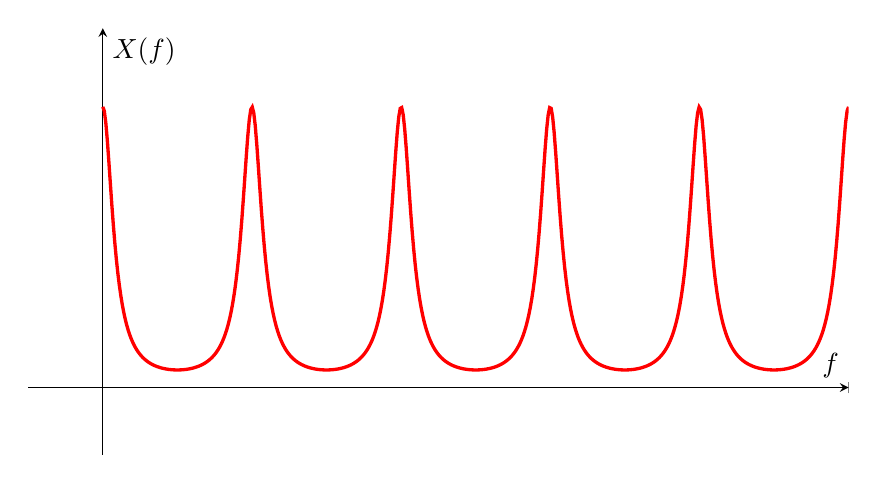
\begin{tikzpicture}
            \begin{axis} [
			axis x line = middle, % The x axis should go through the origin
			axis y line = middle,
			xmin = -1.5,
			xmax = 15,
			ymin = -1.5,
			ymax = 8,
			xlabel = \(f\),
			ylabel = {\(X(f)\)},
			height = 7cm,
			width = 12cm,
			xtick distance=15,
			ytick distance=10,
			xticklabel = \empty
			]
			\addplot[very thick, red, samples = 500, domain = 0:15]{1/((1 + (0.6^2) - 2*0.6 * (cos(x*deg(pi/1.5))))};
			\end{axis}
		\end{tikzpicture}
		}
		\caption{The Amplitude Response of a Comb Filter.}
	\end{center}
\end{figure}

These peaks in the Amplitude Response result in what is described as a ``metallic'' sound, which by itself may not produce a convincing reverb. To achieve a flat frequency response to the comb filter, Schroeder introduces the \textit{Allpass filter} as a method by including an additional feed-forward signal to the output of the comb filter.

\begin{figure}[h] % [h] used to prevent {figure} from doing weird positioning
	\begin{center}
		\framebox[13cm]{%
		\parbox{10.5cm}{
		\begin{tikzpicture}
			% - delay element
			\tikzgrid{
			% building blocks
				\node[input] (in)  {$IN$} & &
				\node[node]  (n1)  {} & &
				\node[delay] (d2) {$-g$} & & & &
				\node[delay] (d1) {$+$} \\ & &
				\node[delay] (g0)  {$+$} & &
				\node[delay] (d0) {DELAY $T$} & &
				\node[node]  (n0)  {} & &
				\node[delay] (d3) {GAIN $1-g^2$} & &
				\node[output] (out) {$OUT$} & \\ & & & &
				\node[delay] (g1) {GAIN $g$} &
			}
			\path[r>] (in) -| (g0);
			\path[r>] (g0) -- (d0);
			\path[r] (d0) -- (n0);
			\path[r>] (n0) |- (g1);
			\path[r>] (g1) -| (g0);
			\path[r>] (n1) -- (d2);
			\path[r>] (d2) -- (d1);
			\path[r>] (n0) -- (d3);
			\path[r>] (d3) -- (d1);
			\path[r>] (d1) -| (out);
		\end{tikzpicture}
		}}
		\caption{The Signal Flow Graph of an Allpass Filter \cite{schroeder1961natural}.}
	\end{center}
\end{figure}

With the additional feed-forward signal $1-g^2$, Schroeder derives the Amplitude Response to be \cite{schroeder1961natural}:
\begin{equation}\label{comb}
	|X(\omega)|=1
\end{equation}

which results in a flat response, removing the ``metallic'' sound of the Comb Filter. With these tools, Schroeder constructs several designs of reverberators that produce sound through purely artificial means. What follows is a description of one such design that he proposes.

% \begin{figure}[h] % [h] used to prevent {figure} from doing weird positioning
% 	\begin{center}
% 		\fbox{
% 		\begin{tikzpicture}
%             \begin{axis} [
% 			axis x line = middle, % The x axis should go through the origin
% 			axis y line = middle,
% 			xmin = -1.5,
% 			xmax = 15,
% 			ymin = -1.5,
% 			ymax = 8,
% 			xlabel = \(f\),
% 			ylabel = {\(X(f)\)},
% 			height = 7cm,
% 			width = 12cm,
% 			xtick distance=15,
% 			ytick distance=10,
% 			xticklabel = \empty
% 			]
% 			\addplot[very thick, red, samples = 10, domain = 0:15]{4};
% 			\end{axis}
% 		\end{tikzpicture}
% 		}
% 		\caption{The Amplitude Response of an Allpass Filter.}
% 	\end{center}
% \end{figure}

\section{The Schroeder Comb Filter Approach}
To achieve a convincing reverb, the \textit{echo density} of the output must be sufficiently large. This measurement is simply the number of echos per second that occur in the resulting output \cite{pirkle2019designing}:
\begin{equation}\label{comb}
	E_D=\frac{echoes}{second}
\end{equation}

According to Schroeder, the echo density must be greater than 1000 to achieve a ``realistic'' sound\footnote{The now-accepted value of sufficient echo density is much higher. In 1989, Griesinger proposed that this value should be 10,000 echoes/second \textit{or higher} due to short impulses providing a ``grainy'' sound, especially for long decay times \cite{griesinger1989practical}. Modern reverberation techniques, however, propose adding a ``diffuser'' step, which removes the graininess that would come from the early reflections of a short impulse. With this additional step, the number of echoes/second can be lowered to 2000-4000 \cite{FiftyYears}.}. To accomplish this, one method he provides is by connecting several Allpass Filters in series, which he postulates can be done with five. This provides an echo density ``sufficiently close'' to the required 1000 \cite{schroeder1961natural}. However, Schroeder goes on to introduce a design that includes both Allpass Filters \textit{and} the aforementioned Comb Filters. Despite the imperfect Amplitude Response of the Comb Filter, Schroeder argues that it may represent real rooms better as they likewise contain irregular responses.

To create a sufficient echo density, a number of Comb Filters of varying delay lengths are connected in parallel before the Allpass Filters in series. In his design, he uses four Comb Filters in parallel with two Allpass Filters in series after. The delay lengths of the Comb Filters are said to be incommensurate in order to prevent regular ``peaks'' from occuring in the output signal \cite{schroeder1961natural}. With this design, a sufficient echo density is created to allow for a reverberation time of approximately one second, similar to what one may find in a real acoustic space. Figure 4.6 provides a Signal Flow Graph of this design.

\begin{figure}[h]
	\begin{center}
	\fbox{
	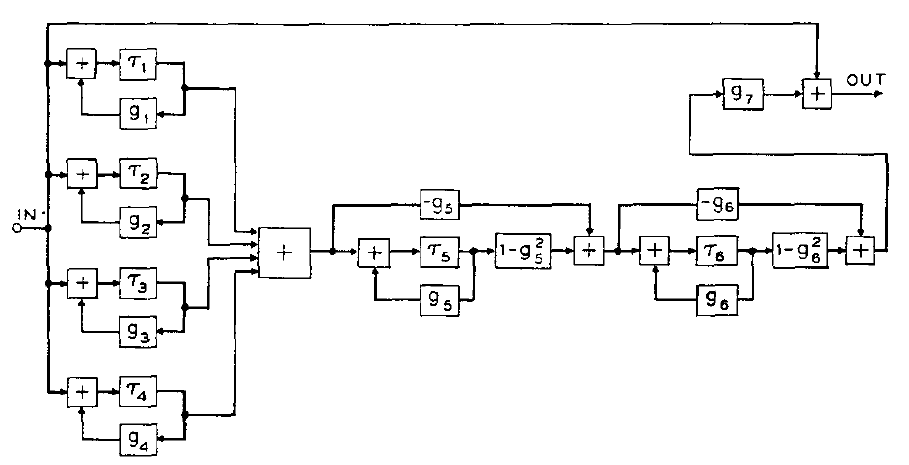
\includegraphics[width=14cm]{figures/schroeder.png}
	}
	\caption{A Signal Flow Graph of Schroeder's Reverberator using Comb Filters and Allpass Filters \cite{schroeder1961natural}.}
	\end{center}
\end{figure}

Many artificial reverberation designs use similar principles of repeating the given input signal but can differ in what or how many filters are used. One of the first open-source designs, \textit{Freeverb}\footnote{Interestingly, Freeverb predates a large majority of Open Source Software, as its source code was released publicly on May 24th, 2000 \cite{freeverb}.}, used four Allpass Filters in series and eight parallel Filtered-Feedback Comb Filters (or rather, a Comb Filter with a Lowpass Filter placed in the feedback loop) \cite{PASPWEB2010}. For each of the designs provided, channels of audio are processed under a single mono channel of audio data. As will be discussed in Chapter 8, splitting audio data into multiple channels is another method of creating a greater echo density.

\section{Convolution}
Convolution is a fundamentally different approach to the Schroeder Comb Filter Approach. Unlike Comb Filters and Allpass Filters, they involve taking an input signal and manipulating it with a particular \textit{impulse response}. In doing so, the two signals are combined (or convolved, rather) such that the output signal contains the product of the input signal and the state of the room measured \cite{pirkle2019designing}. While room responses are useful to convolve with, there is nothing stopping one from convolving one signal $x(n)$ with any other arbitrary signal $y(n)$. For discrete signals, the multiplication of Discrete Fourier Transforms (Definition 4.3) correspond to \textit{circular convolution}, which is defined by the following (under the time domain):

\makeatletter
\newcommand\xleftrightarrow[2][]{%
  \ext@arrow 9999{\longleftrightarrowfill@}{#1}{#2}}
\newcommand\longleftrightarrowfill@{%
  \arrowfill@\leftarrow\relbar\rightarrow}
\makeatother

\begin{defn}[Definition of Circular Convolution \cite{wolfsound}]\label{def-cir-FT}
	\begin{equation}\label{eq-cir-FT)}
	x(n) \circledast y(n) \xleftrightarrow{\text{DFT}} X(k)Y(k)
	\end{equation}
	\begin{equation}\label{next-ig}
	x(n) \circledast y(n) = \sum_{m=0}^{N-1} x(m) y[(m - n) \% N]
	\end{equation}
\end{defn}

where $\circledast$ refers to the process of convolving a signal under the time domain, and $X(k)Y(k)$ are the corresponding signals under the frequency domain (similar to that of the Amplitude Responses mentioned earlier). In an intuitive sense, this process can be described as the ``sliding'' of the impulse response over the input to create overlapping areas \cite{pirkle2019designing}. The area under these signals are then computed for each iteration of the slide, resulting in an output signal that is the convolution between the two. Figure 4.7 describes this process visually.

\begin{figure}[h]
	\begin{center}
	\fbox{
	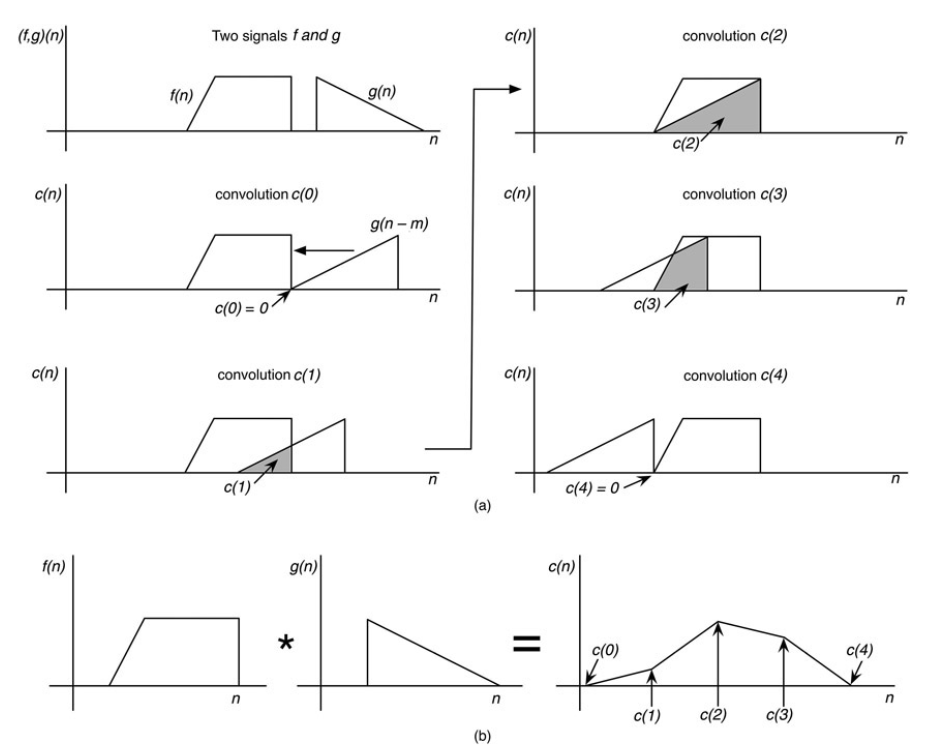
\includegraphics[width=12cm]{figures/TO-REPLACE.png}
	}
	\caption{A visual representation of two waveforms being convolved \cite{pirkle2019designing}.}
	\end{center}
\end{figure}

In simpler terms, Convolution is the process of computing the Fourier Transform of a particular input signal and - in the context of artificial reverberation - the impulse response of a room, multiplying the two signals together such that their frequency responses match what one would hear if the signals were combined (as opposed to played at the same time), and then computing the inverse DFT (summing the output of the DFT back together again). In theory, this process seems quite simple and extremely powerful; in practice, the implementation of the above process is difficult due to the sheer number of computations required \cite{pirkle2019designing}. Put simply, the shorter the impulse response, the less computations required to convolve the provided input signal.
